\section{Mission Lifecycle and Durable State}
\label{sec:lifecycle}\label{sec:runtime}\label{sec:state}

\begin{designbox}
Run one mission at a time, back to back, for days --- surviving restarts, upgrades,
and provider outages --- without ever re-deciding a committed campaign or killing a
mission mid-flight. Keep the durable truth on disk: the append-only event tape is
the system of record, and every other file is a derivable view. Provider sessions
are bounded caches, not the sole memory.
\end{designbox}

The runtime is the 7$\times$24 loop that turns a durable objective into a stream of
missions. Figure~\ref{fig:lifecycle} shows the lifecycle and its recovery edges.
This section describes the states, the process model, the restart/resume semantics,
and the on-disk state that together make a long campaign durable.

\begin{figure}[ht]
\centering
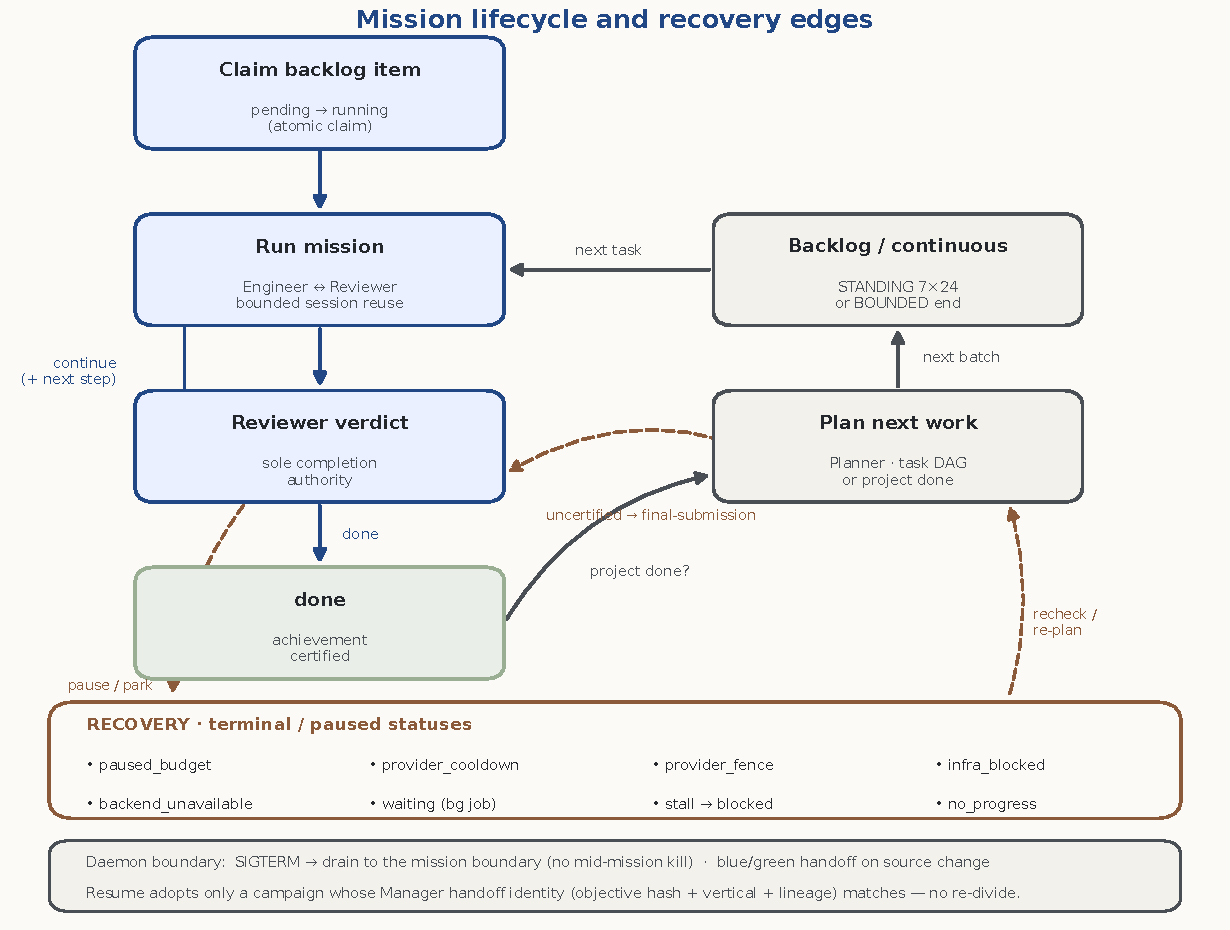
\includegraphics[width=0.9\textwidth]{figures/mission_lifecycle.pdf}
\caption{Mission lifecycle and recovery edges. The primary spine (indigo) claims a
backlog item, runs an Engineer$\leftrightarrow$Reviewer mission, and acts on the
Reviewer verdict; the plan-next loop (grey) refills the backlog; recovery edges
(terracotta) route paused and blocked missions to first-class statuses and back. The
daemon boundary governs draining, handoff, and identity-checked resume.}
\label{fig:lifecycle}
\end{figure}

\subsection{From backlog claim to mission outcome}

The \code{LifeSupervisor} runs a synchronous outer loop: it claims the next backlog
item, injects a non-authoritative recency memory preamble without polluting the raw
objective, runs the mission through the execution plane, accounts the cost against
budget gates, writes a journal entry, and --- when the backlog empties in continuous
mode --- invokes the Planner for the next batch. The backlog claim
(\code{pending}$\rightarrow$\code{running}) is atomic, so two workers can never take
the same item; orphaned \code{running} items from a prior crash are reaped on
startup. The loop is deliberately synchronous --- one mission at a time --- which is
what makes the mission boundary a clean, well-defined point for stopping, upgrading,
and resuming.

Every mission ends in a first-class terminal or paused status, never an unbounded
spin. Terminal outcomes include \code{done}, \code{blocked}, \code{max\_rounds},
\code{no\_progress}, and \code{error}; paused outcomes include \code{paused\_budget},
\code{paused\_provider\_cooldown}, \code{paused\_provider\_fence}, and
\code{infra\_blocked} (full taxonomy in Appendix~\ref{app:status}). A paused mission
is not a failure --- it records that the campaign is correctly waiting on an external
condition. Separately, a \code{replan\_requested} status is a \emph{control
transfer} back to the Planner, not a successful completion and not a
done/failed/blocked outcome: the current item returns to \code{pending} and then
passes the normal Planner rate and budget gate before any re-plan takes effect.

\subsection{Persisted identity and safe resume}

For unattended operation the runtime runs as a detached daemon worker
(\srcpath{daemon/life\_worker.py}, roughly 1{,}800 lines) wrapping the supervisor.
On \code{SIGTERM} or \code{SIGINT} it drains to the next mission-tick boundary rather
than interrupting a live mission, so an in-progress evaluation or a result being
recorded is never severed. A run is protected by both the atomic backlog claim and a
per-project \code{daemon.pid} lock, so a second daemon cannot drive the same project.

A 7$\times$24 system must be upgradable without losing a campaign. Argus handles a
source change with a \textbf{blue/green self-handoff}: the worker detects a change in
its own source signature, spawns a candidate child under a handoff protocol with a
bounded generation count and a minimum inter-handoff interval, and hands the campaign
over at a clean boundary (\srcpath{daemon/handoff.py}). The Manager-to-daemon handoff
\emph{identity} (objective hash, vertical, lineage generation) is persisted and
recoverable from the immutable event tape. Resume is identity-checked: a
\code{--resume-continuous} start adopts only a persisted campaign whose identity
matches; a mismatched or missing identity forces a real Manager division rather than
blindly re-attaching. Crash and reboot restart is owned by the \code{systemd --user}
unit (Section~\ref{sec:operations}) plus \code{loginctl enable-linger}, not bespoke
keep-alive logic.

\subsection{Bounded sessions and curated working memory}

Argus does \emph{not} depend on one unbounded provider transcript. The Engineer and
Reviewer use separate resumable sessions, so recent context and provider prefix
caches stay useful, while a structured \code{checkpoint.json} in the project state
directory carries curated cross-round state (\srcpath{engineer/checkpoint.py},
\srcpath{apps/\_runtime.py}). Its \code{CheckpointState} fields cover the goal,
verified work, dead ends, one open blocker, the next step, and bounded environment
facts. The \emph{Reviewer} authors it: the Engineer ends a turn with a concise
handoff proposal, and the Reviewer validates that proposal against the artifacts and
writes the canonical checkpoint by atomic rewrite. Python enforces hard item and
character caps --- not only in the prompt or schema --- so the checkpoint stays a
\emph{current-state} object rather than an append-only log; stale detail is deleted
while ground truth remains in on-disk artifacts.

The resume window is explicitly bounded. By default the runtime rolls each role's
thread after three rounds on that thread, or when the preceding call reports at least
1.5 million input tokens; the next call opens a new session and the Engineer is
reseeded from the checkpoint (\srcpath{engineer/runner.py}, \srcpath{core/knobs.py}).
If provider-side compaction occurs before a roll, the next round resends the full
static preamble. This combines short-window context reuse with a structural limit on
transcript growth, and it fails soft: a missing or garbled checkpoint keeps the last
good one rather than clearing memory.

\subsection{The on-disk state map}

Core path helpers define the global and per-project roots (\srcpath{core/paths.py});
runtime composition derives the checkpoint path inside the project state directory
(\srcpath{apps/\_runtime.py}). A global root \code{\textasciitilde/.argus-skill/}
(overridable via \code{ARGUS\_SKILL\_HOME}) holds cross-project identity, shared
skills, and an operator knob store; each project lives under
\code{projects/<fingerprint>/}. Table~\ref{tab:persist} lists the principal state
files, their owner, and their mutability. The canonical timeline is the append-only
\code{events.jsonl}; every other file is a derived view or working state that can be
rebuilt or safely reset.

\begin{table}[t]
\centering
\small
\begin{tabularx}{\linewidth}{@{}p{3.4cm} p{2.2cm} X p{1.9cm}@{}}
\toprule
\textbf{Path (per project)} & \textbf{Owner} & \textbf{Content} & \textbf{Mutability} \\
\midrule
\code{events.jsonl}        & evidence plane & canonical typed-event timeline & append-only \\
\code{backlog.jsonl}       & scheduler      & pending / running / done work items & atomic claim \\
\code{continuous.json}     & scheduler      & STANDING lifetime + campaign config & rewrite \\
\code{inbox.jsonl}         & operator       & queued operator messages / answers & append + drain \\
\code{checkpoint.json}     & Reviewer       & hard-capped curated working memory & atomic rewrite \\
\code{daemon.pid}          & daemon         & concurrency lock & exclusive \\
\code{daemon.status.json}  & daemon         & liveness / status snapshot & rewrite \\
\addlinespace
\code{identity.md}$^\dagger$ & global & author / machine identity & operator \\
\code{skills/}$^\dagger$     & global & shared skill library & versioned \\
\code{config.json}$^\dagger$ & global & operator knob overrides & operator \\
\bottomrule
\end{tabularx}
\caption{Principal persisted state (abridged; full map in
Appendix~\ref{app:state}). The event tape is the only append-only source of truth;
everything else is derivable or resettable. $^\dagger$ under the global root
\code{\textasciitilde/.argus-skill/}.}
\label{tab:persist}
\end{table}

Long-term knowledge lives in two systems on this state. Skills are versioned Markdown
files distilled on a matcher miss and revised from real usage (\srcpath{skills/}); a
per-project wiki records an immutable \emph{source} RoundCard after each Reviewer
verdict, from which the Reviewer may later synthesize evidence-cited pages
(Section~\ref{sec:evidence}). Both compound capability across missions without
becoming an unbounded prompt.
